\documentclass[../main.tex]{subfiles}
\usetikzlibrary{shapes, arrows.meta, positioning}
\begin{document}

\subsection{Password file} Juels and Rivest \cite{juels2013honeywords} assume
in their paper that a system on which users have to log in with a password. Each
user has an entry \(c_i\) in the password file. A good example is the password
files of an unix-like system /etc/passwd \cite{passwd} and /etc/shadow
\cite{shadow}. They store the username \(u_i\), the hash of the password
\(H(p_i)\), and additional information about the user. \[c_i = (u_i, H(p_i))\]

Honeywords as explained in the introduction section are decoy passwords,
therefore when using this method, the password file will have up to \(k\)
passwords attached to each entry. Let \(S_i\) be the set of the correct
password and all decoy passwords of the user \(u_i\), the set will be called
sugarwords. \[S_i = {H(p_0), H(p_1), ..., H(p_k)}\]. Thus, an entry \(c_i\)
in the password file will be defined as follows: \[c_i = (u_i, S_i)\]

The hashed passwords should be hashed with an additional salt. Salt is extra
information which is usually a randomly generated string concatenated to the
password, the resulting string is hashed. It is recommended to use one salt per
user. If not salted passwords are easily brute forceable which makes the system
more prone to attacks. After salting, the adversary has a larger set of strings
to test to get the same hash. To make it more clear you can look at the
examples provided in table \ref{table:1} and \ref{table:2}.


\begin{table}
  \centering
	\begin{tabularx}{0.5\textwidth}{|X|X|X|}
    \hline \textbf{Username} & \textbf{Plain password} & \textbf{Hashed password using SHA256} \\ \hline
    Bob & bob123 & 8d059c3640b97180
		   dd2ee453e20d34ab
		   0cb0f2eccbe87d01
		   915a8e578a202b11\\
    \hline
    Alice & alice123 & 4e40e8ffe0ee32fa
		       53e139147ed55922
		       9a5930f89c220470
		       6fc174beb36210b3\\
    \hline
  \end{tabularx}
  \caption{Hashed password without salt}
  \label{table:1}
\end{table}

\begin{table}
  \centering
	\begin{tabularx}{0.5\textwidth}{|m{0.15\linewidth}|m{0.15\linewidth}|m{0.2\linewidth}
		|X|}
    \hline
		\textbf{Username} & \textbf{Plain password} & \textbf{salt} &
    \textbf{Hashed password using SHA256} \\ 
    \hline
    Bob & bob123     & PqaH7b9P & d79fe7c073f3a081
			          e81b7e230c54124f
			          0b11484508cd961d
			          349436f9d4ef1e45\\
    \hline
    Alice & alice123 & T2dYghL3 & 8988d499b23ee3d9
		                  0f3240f10f1cb48e
				  0387701de5ef41d1
				  4100960ab007a203\\
    \hline
  \end{tabularx}
  \caption{Hashed password with salt}
  \label{table:2}
\end{table}


\subsection{Honeychecker}
The goal of using Honeywords is to alarm the system administrator that the
password file is compromised. If the password file is compromised, one should
assume that the system holding the file is also exposed to an adversary. This
implies that the adversary has potential knowledge or even control over the
alarm mechanism if it is programmed in this same system. To overcome this,
Juels and Rivest suggest a distributed security system consisting of a separate
hardened computer called a honeychecker. The honeychecker should detect
abnormalities and raise an alarm if the password file is breached.

The honeychecker stores a single number \(n_i\) in its database for each user
and it will never receive or store the password itself. The number \(n_i\) is
in the range of \(1 to k\), \(k\) being the number of sugarwords of the user
\(u_i\). The honeychecker will have two functions, the first being:

\[Set(i,j)\]

The function takes as parameters the index of a user \(i\) and a new index of
the correct password \(j\). It sets \(n_i = j\). The second function is:

\[Check(i,j)\]

The function takes as parameters also the index of the user \(i\) and an index
of a password \(j\). The honeychecker has to check whether \(n_i\) is equal to
\(j\).

An advantage of this distributed security system is, that if the honeychecker is
compromised, the password has the same security level as if the honeychecker
did not exist.

In figure \ref{fig:Figure 1} you see a flowchart depicting a login process.
First, the user tries to log in with a password \(p\). The system checks if \(p
\in S_i\); if not the system has a choice between several policies on what to do,
in the case of a user entering the wrong password. If \(p \in S_i\), the system
sends \(i\) to the honeychecker \(H\). \(H\) then checks, if the password is
the correct one of the sugarwords. If it returns false, it raises an alarm, and the
system administrator then again has several policies to choose from when such an
alarm occurs. An example is a honeypot, where the user is directed to a
decoy screen with restricted access. When the honeychecker returns true, it
sends a confirmation to the system. After that, the user is granted access. 

\begin{figure}
  \centering
    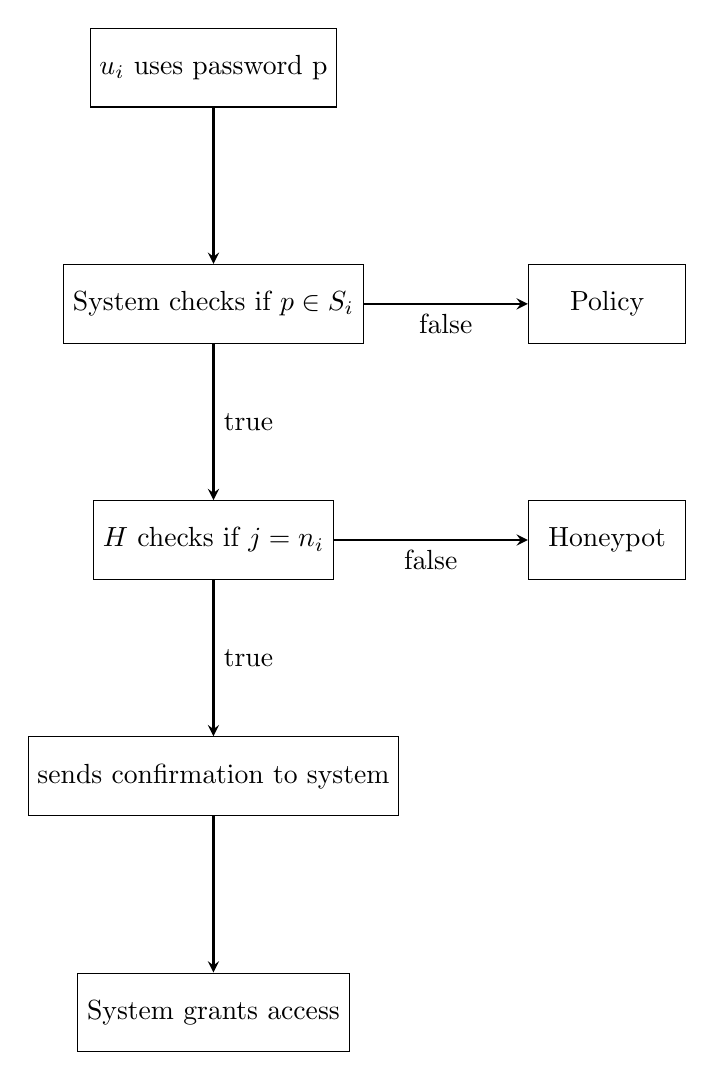
\begin{tikzpicture}[node distance=1.5cm]
    \tikzstyle{startstop} = [rectangle, draw, minimum width=2cm, minimum height=1cm, text centered, node distance=3cm]
    \tikzstyle{process} = [rectangle, draw, text centered, minimum width=2cm, minimum height=1cm, node distance=3cm]
    \tikzstyle{decision} = [rectangle, draw, text centered, minimum width=2cm, minimum height=1cm, node distance=3cm]
    \tikzstyle{arrow} = [thick,->,>=stealth]

    \node (start) [startstop] {\(u_i\) uses password p};
    \node (init) [process, below of=start] {System checks if \(p \in S_i\)};
    \node (authenticate) [process, below of=init] {\(H\) checks if \(j = n_i\)};
    \node (decision) [decision, below of=authenticate] {sends confirmation to system};
    \node (access) [process, below of=decision] {System grants access};
    \node (policy) [process, right of=init, xshift=2cm] {Policy};
    \node (honeypot) [process, right of=authenticate, xshift=2cm] {Honeypot};

    % Arrows
    \draw [arrow] (start) -- (init);
    \draw [arrow] (init) -- node[anchor=west] {true}(authenticate);
	    \draw [arrow] (init) -- node[anchor=north] {false}(policy);
    \draw [arrow] (authenticate) -- node[anchor=west] {true}(decision);
    \draw [arrow] (authenticate) -- node[anchor=north] {false}(honeypot);
    \draw [arrow] (decision) -- (access);
  \end{tikzpicture}
  \caption{Honeychecker Login Flowchart}
  \label{fig:Figure 1}
\end{figure}

The change or create process is represented in \ref{fig:Figure 2}. In both
processes the user \(u_i\) starts with sending a request to the server. The
server then generates \(k-1\) honeywords according to the given password \(p\)
with help of a generating method \(Gen(p)\). Generating methods are going to be
looked at in detail in the following section. The function returns the resulting
set of sugarwords \(S_i\). After, that it sends the index of the correct
password \(j\) to the honeychecker\(H\). The honeychecker \(H\) then uses its'
\(Set(i,j)\) function explained above, then confirms the change/create of the
index to the server. The server then updates the entry \(c_i\) with the new
sugarwords.

\begin{figure}
  \centering
    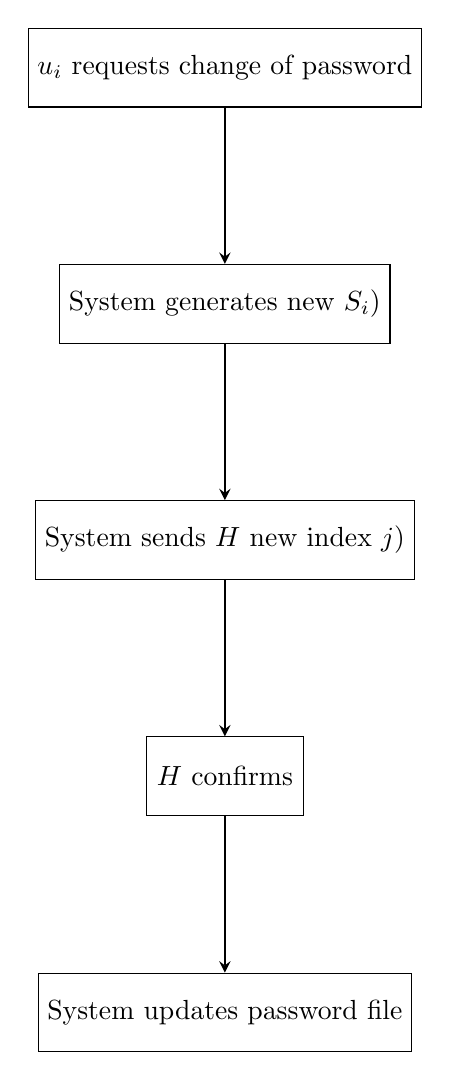
\begin{tikzpicture}[node distance=1.5cm]
    \tikzstyle{startstop} = [rectangle, draw, minimum width=2cm, minimum height=1cm, text centered, node distance=3cm]
    \tikzstyle{process} = [rectangle, draw, text centered, minimum width=2cm, minimum height=1cm, node distance=3cm]
    \tikzstyle{decision} = [rectangle, draw, text centered, minimum width=2cm, minimum height=1cm, node distance=3cm]
    \tikzstyle{arrow} = [thick,->,>=stealth]

    \node (start) [startstop] {\(u_i\) requests change of password};
    \node (init) [process, below of=start] {System generates new \(S_i\))};
    \node (authenticate) [process, below of=init] {System sends \(H\) new index \(j\))};
    \node (decision) [decision, below of=authenticate] {\(H\) confirms};
    \node (access) [process, below of=decision] {System updates password file};

    % Arrows
    \draw [arrow] (start) -- (init);
    \draw [arrow] (init) -- (authenticate);
    \draw [arrow] (authenticate) -- (decision);
    \draw [arrow] (decision) -- (access);
  \end{tikzpicture}
  \caption{Honeychecker Change/Create Flowchart}
  \label{fig:Figure 2}
\end{figure}

\subsection{Generation methods}

Juels and Rivest propose several methods for generating decoy passwords, such
that it is hard to guess the correct password in case the adversary knows all
the sugarwords. The goal of a good method is to be flat, meaning that when the
adversary knows all \(k\) sugarwords \(S_i\) of some user \(u_i\). The
probability that he chooses the correct one is \[P = 1/k\].  

There are two different categories legacy-UI password and modified-UI approach.
With legacy-UI password approaches just have to tell the system their new
password. With the help of this password, the honeywords are generated. The benefit
of this approach is that the user does not need to know that honeywords are
generated. The report looks at two methods and an additional hardening of such
methods:

\begin{itemize}
  \item Chaffing by tweaking
  \item Chaffing with a password model
  \item Use of "tough nuts"
\end{itemize}

On the other hand with modified-UI approaches the user is asked
again for some extra intervention for example appending three random generated
numbers, such methods make it easier to prove the flatness of a method. The report will
look at the "take-a-tail" method as an example.

\subsubsection{Chaffing by tweaking}

Chaffing by tweaking involves changing specific positions of
strings, such that digits are replaced by digits, letters by letters, and
special characters by special characters. The character is replaced by a random
character. Examples of such methods are chaffing-by-tail-tweaking and
chaffing-by-tweaking-digits. It is important to note that one should only
change patterns of characters because it could become obvious to distinguish
the real password if one changes specific characters of a word for example. The flatness
of this method relies on the user, if the tweaked positions are also randomly chosen by
the user implies perfect flatness.

\subsubsection{Chaffing with a password model}

This model generates honeywords using a large set of real passwords. Although
using a public list might give the adversary to exploit the list to his
advantage. A simple example approach using this method would be splitting
the given password into separate words and replacing the words with the help of a
large set of words. When replacing the words one would replace 4-letter words
with 4-letter words and n-letter words with n-letter words.

\subsubsection{Use of tough nuts}
Tough nuts are honeywords that are very hard to impossible to crack. This can
improve the security of chaffing algorithms. By incorporating several tough
nuts, the adversary cannot know if the passwords are among the tough
nuts or the rest. Thus, making it harder for him to guess the correct password.

\subsubsection{Take-a-tail}
This method is an example of a modified-UI change approach. When the user enters
a new password, the system generates a random tail for example three numbers, and
asks the user to remember and append them to their password. This ensures that the
adversary can't distinguish between the honeywords and the password.

\end{document}
